\documentclass{standalone}
\usepackage{tikz}
\usetikzlibrary{patterns, positioning}

\begin{document}
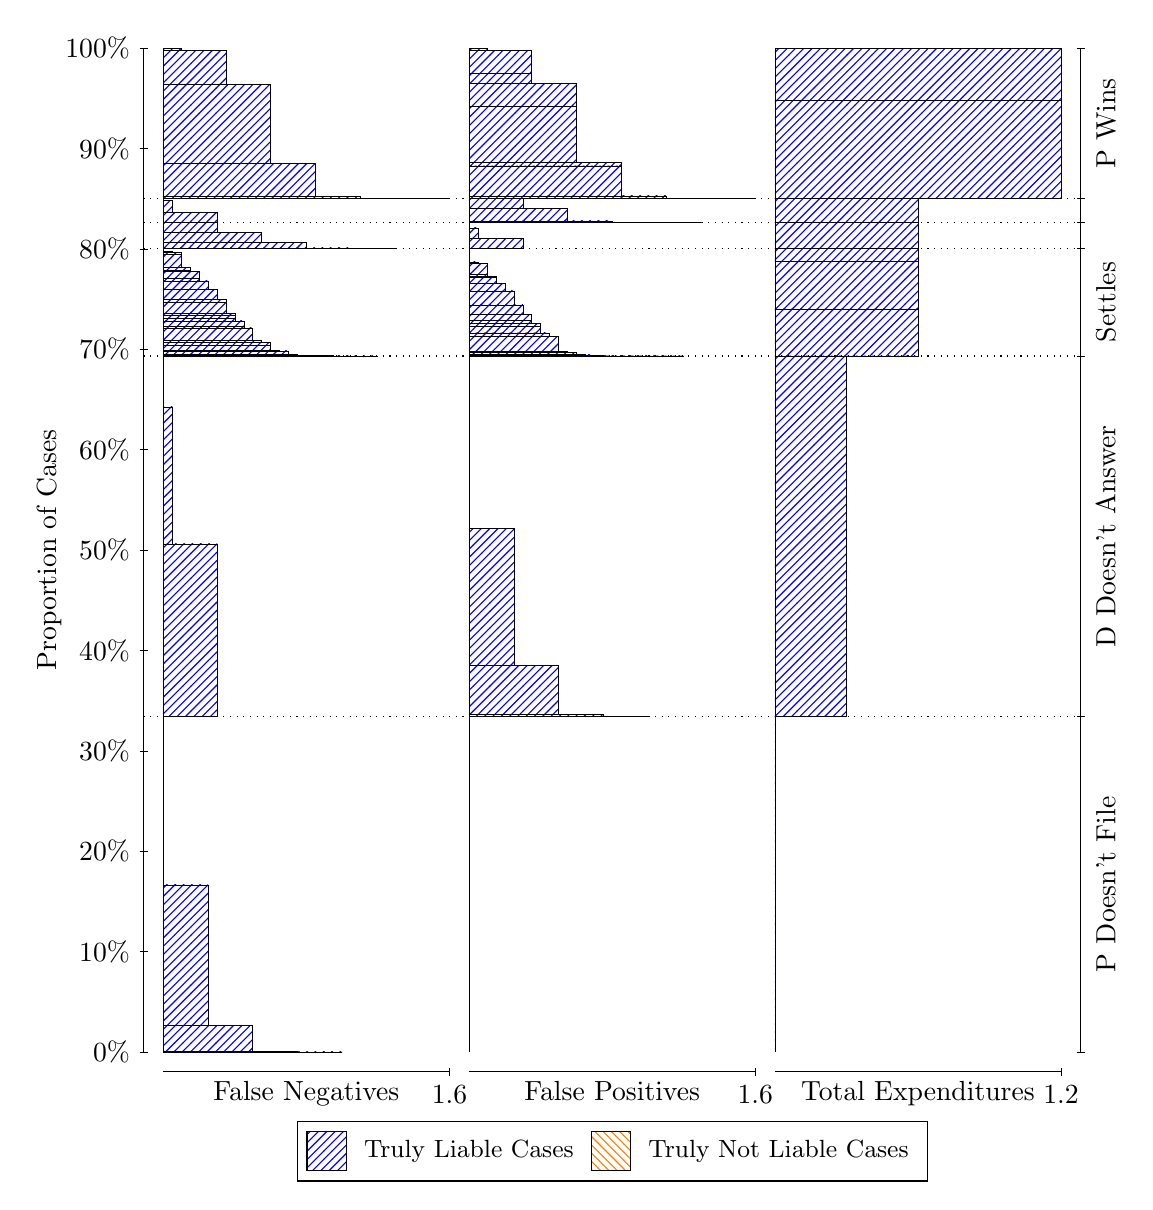
\begin{tikzpicture}
\draw[black, very thin] (1.5,1.75) -- (1.5,14.5);
\node[rotate=90, anchor=center] at (0.3, 8.125) {Proportion of Cases};
\draw[black, very thin] (1.45,1.75) -- (1.55,1.75);
\node[anchor=east] at (1.45, 1.75) {0\%};
\draw[black, very thin] (1.45,3.025) -- (1.55,3.025);
\node[anchor=east] at (1.45, 3.025) {10\%};
\draw[black, very thin] (1.45,4.3) -- (1.55,4.3);
\node[anchor=east] at (1.45, 4.3) {20\%};
\draw[black, very thin] (1.45,5.575) -- (1.55,5.575);
\node[anchor=east] at (1.45, 5.575) {30\%};
\draw[black, very thin] (1.45,6.85) -- (1.55,6.85);
\node[anchor=east] at (1.45, 6.85) {40\%};
\draw[black, very thin] (1.45,8.125) -- (1.55,8.125);
\node[anchor=east] at (1.45, 8.125) {50\%};
\draw[black, very thin] (1.45,9.4) -- (1.55,9.4);
\node[anchor=east] at (1.45, 9.4) {60\%};
\draw[black, very thin] (1.45,10.675) -- (1.55,10.675);
\node[anchor=east] at (1.45, 10.675) {70\%};
\draw[black, very thin] (1.45,11.95) -- (1.55,11.95);
\node[anchor=east] at (1.45, 11.95) {80\%};
\draw[black, very thin] (1.45,13.225) -- (1.55,13.225);
\node[anchor=east] at (1.45, 13.225) {90\%};
\draw[black, very thin] (1.45,14.5) -- (1.55,14.5);
\node[anchor=east] at (1.45, 14.5) {100\%};

\draw[black, very thin] (13.4,1.75) -- (13.4,14.5);
\draw[black, very thin] (13.35,1.75) -- (13.45,1.75);
\node[anchor=west] at (13.35, 1.75) {};
\draw[black, very thin] (13.35,6.0109) -- (13.45,6.0109);
\node[anchor=west] at (13.35, 6.0109) {};
\draw[black, very thin] (13.35,10.589) -- (13.45,10.589);
\node[anchor=west] at (13.35, 10.589) {};
\draw[black, very thin] (13.35,11.959) -- (13.45,11.959);
\node[anchor=west] at (13.35, 11.959) {};
\draw[black, very thin] (13.35,12.285) -- (13.45,12.285);
\node[anchor=west] at (13.35, 12.285) {};
\draw[black, very thin] (13.35,12.587) -- (13.45,12.587);
\node[anchor=west] at (13.35, 12.587) {};
\draw[black, very thin] (13.35,14.5) -- (13.45,14.5);
\node[anchor=west] at (13.35, 14.5) {};

\draw[black, very thin, pattern color=blue, pattern=north east lines] (1.75,1.75) rectangle (4.0208,1.75);
\draw[black, very thin, pattern color=blue, pattern=north east lines] (1.75,1.75) rectangle (3.4531,1.7529);
\draw[black, very thin, pattern color=blue, pattern=north east lines] (1.75,1.7529) rectangle (2.8854,2.0883);
\draw[black, very thin, pattern color=blue, pattern=north east lines] (1.75,2.0883) rectangle (2.3177,3.8721);
\draw[black, very thin, pattern color=orange, pattern=north west lines] (1.75,3.8721) rectangle (1.75,3.8721);
\draw[black, very thin, pattern color=blue, pattern=north east lines] (1.75,3.8721) rectangle (1.75,6.0109);
\draw[black, very thin, pattern color=blue, pattern=north east lines] (1.75,6.0109) rectangle (2.4312,8.2016);
\draw[black, very thin, pattern color=blue, pattern=north east lines] (1.75,8.2016) rectangle (1.8635,9.9434);
\draw[black, very thin, pattern color=orange, pattern=north west lines] (1.75,9.9434) rectangle (1.75,9.9434);
\draw[black, very thin, pattern color=blue, pattern=north east lines] (1.75,9.9434) rectangle (1.75,10.589);
\draw[black, very thin, pattern color=blue, pattern=north east lines] (1.75,10.589) rectangle (4.475,10.589);
\draw[black, very thin, pattern color=blue, pattern=north east lines] (1.75,10.589) rectangle (4.2479,10.589);
\draw[black, very thin, pattern color=blue, pattern=north east lines] (1.75,10.589) rectangle (4.0208,10.589);
\draw[black, very thin, pattern color=blue, pattern=north east lines] (1.75,10.589) rectangle (3.9073,10.592);
\draw[black, very thin, pattern color=blue, pattern=north east lines] (1.75,10.592) rectangle (3.7937,10.592);
\draw[black, very thin, pattern color=blue, pattern=north east lines] (1.75,10.592) rectangle (3.7937,10.592);
\draw[black, very thin, pattern color=blue, pattern=north east lines] (1.75,10.592) rectangle (3.6802,10.595);
\draw[black, very thin, pattern color=blue, pattern=north east lines] (1.75,10.595) rectangle (3.5667,10.596);
\draw[black, very thin, pattern color=blue, pattern=north east lines] (1.75,10.596) rectangle (3.4531,10.606);
\draw[black, very thin, pattern color=blue, pattern=north east lines] (1.75,10.606) rectangle (3.3396,10.654);
\draw[black, very thin, pattern color=blue, pattern=north east lines] (1.75,10.654) rectangle (3.226,10.659);
\draw[black, very thin, pattern color=blue, pattern=north east lines] (1.75,10.659) rectangle (3.226,10.664);
\draw[black, very thin, pattern color=blue, pattern=north east lines] (1.75,10.664) rectangle (3.1125,10.72);
\draw[black, very thin, pattern color=blue, pattern=north east lines] (1.75,10.72) rectangle (3.1125,10.763);
\draw[black, very thin, pattern color=blue, pattern=north east lines] (1.75,10.763) rectangle (2.999,10.784);
\draw[black, very thin, pattern color=blue, pattern=north east lines] (1.75,10.784) rectangle (2.8854,10.946);
\draw[black, very thin, pattern color=blue, pattern=north east lines] (1.75,10.946) rectangle (2.7719,10.965);
\draw[black, very thin, pattern color=blue, pattern=north east lines] (1.75,10.965) rectangle (2.7719,11.034);
\draw[black, very thin, pattern color=blue, pattern=north east lines] (1.75,11.034) rectangle (2.6583,11.072);
\draw[black, very thin, pattern color=blue, pattern=north east lines] (1.75,11.072) rectangle (2.6583,11.102);
\draw[black, very thin, pattern color=blue, pattern=north east lines] (1.75,11.102) rectangle (2.6583,11.132);
\draw[black, very thin, pattern color=blue, pattern=north east lines] (1.75,11.132) rectangle (2.5448,11.271);
\draw[black, very thin, pattern color=blue, pattern=north east lines] (1.75,11.271) rectangle (2.5448,11.31);
\draw[black, very thin, pattern color=blue, pattern=north east lines] (1.75,11.31) rectangle (2.4312,11.43);
\draw[black, very thin, pattern color=blue, pattern=north east lines] (1.75,11.43) rectangle (2.3177,11.543);
\draw[black, very thin, pattern color=blue, pattern=north east lines] (1.75,11.543) rectangle (2.2042,11.58);
\draw[black, very thin, pattern color=blue, pattern=north east lines] (1.75,11.58) rectangle (2.2042,11.666);
\draw[black, very thin, pattern color=blue, pattern=north east lines] (1.75,11.666) rectangle (2.0906,11.671);
\draw[black, very thin, pattern color=blue, pattern=north east lines] (1.75,11.671) rectangle (2.0906,11.68);
\draw[black, very thin, pattern color=blue, pattern=north east lines] (1.75,11.68) rectangle (2.0906,11.71);
\draw[black, very thin, pattern color=blue, pattern=north east lines] (1.75,11.71) rectangle (1.9771,11.881);
\draw[black, very thin, pattern color=blue, pattern=north east lines] (1.75,11.881) rectangle (1.9771,11.902);
\draw[black, very thin, pattern color=blue, pattern=north east lines] (1.75,11.902) rectangle (1.8635,11.915);
\draw[black, very thin, pattern color=orange, pattern=north west lines] (1.75,11.915) rectangle (1.75,11.915);
\draw[black, very thin, pattern color=blue, pattern=north east lines] (1.75,11.915) rectangle (1.75,11.959);
\draw[black, very thin, pattern color=blue, pattern=north east lines] (1.75,11.959) rectangle (4.7021,11.959);
\draw[black, very thin, pattern color=blue, pattern=north east lines] (1.75,11.959) rectangle (4.1344,11.962);
\draw[black, very thin, pattern color=blue, pattern=north east lines] (1.75,11.962) rectangle (3.5667,12.027);
\draw[black, very thin, pattern color=blue, pattern=north east lines] (1.75,12.027) rectangle (2.999,12.16);
\draw[black, very thin, pattern color=blue, pattern=north east lines] (1.75,12.16) rectangle (2.4312,12.285);
\draw[black, very thin, pattern color=orange, pattern=north west lines] (1.75,12.285) rectangle (1.75,12.285);
\draw[black, very thin, pattern color=blue, pattern=north east lines] (1.75,12.285) rectangle (2.4312,12.413);
\draw[black, very thin, pattern color=blue, pattern=north east lines] (1.75,12.413) rectangle (1.8635,12.568);
\draw[black, very thin, pattern color=orange, pattern=north west lines] (1.75,12.568) rectangle (1.75,12.568);
\draw[black, very thin, pattern color=blue, pattern=north east lines] (1.75,12.568) rectangle (1.75,12.587);
\draw[black, very thin, pattern color=blue, pattern=north east lines] (1.75,12.587) rectangle (5.3833,12.587);
\draw[black, very thin, pattern color=blue, pattern=north east lines] (1.75,12.587) rectangle (4.8156,12.588);
\draw[black, very thin, pattern color=blue, pattern=north east lines] (1.75,12.588) rectangle (4.2479,12.619);
\draw[black, very thin, pattern color=blue, pattern=north east lines] (1.75,12.619) rectangle (3.6802,13.036);
\draw[black, very thin, pattern color=blue, pattern=north east lines] (1.75,13.036) rectangle (3.1125,14.038);
\draw[black, very thin, pattern color=blue, pattern=north east lines] (1.75,14.038) rectangle (2.5448,14.467);
\draw[black, very thin, pattern color=blue, pattern=north east lines] (1.75,14.467) rectangle (1.9771,14.5);
\draw[black, very thin, pattern color=orange, pattern=north west lines] (1.75,14.5) rectangle (1.75,14.5);
\draw[black, very thin, pattern color=blue, pattern=north east lines] (1.75,14.5) rectangle (1.75,14.5);
\draw[black, very thin, pattern color=orange, pattern=north west lines] (5.6333,1.75) rectangle (5.6333,1.75);
\draw[black, very thin, pattern color=blue, pattern=north east lines] (5.6333,1.75) rectangle (5.6333,6.0109);
\draw[black, very thin, pattern color=orange, pattern=north west lines] (5.6333,6.0109) rectangle (7.9042,6.0109);
\draw[black, very thin, pattern color=blue, pattern=north east lines] (5.6333,6.0109) rectangle (7.9042,6.011);
\draw[black, very thin, pattern color=blue, pattern=north east lines] (5.6333,6.011) rectangle (7.3365,6.0402);
\draw[black, very thin, pattern color=blue, pattern=north east lines] (5.6333,6.0402) rectangle (6.7687,6.6569);
\draw[black, very thin, pattern color=blue, pattern=north east lines] (5.6333,6.6569) rectangle (6.201,8.3987);
\draw[black, very thin, pattern color=blue, pattern=north east lines] (5.6333,8.3987) rectangle (5.6333,10.589);
\draw[black, very thin, pattern color=orange, pattern=north west lines] (5.6333,10.589) rectangle (8.3583,10.589);
\draw[black, very thin, pattern color=blue, pattern=north east lines] (5.6333,10.589) rectangle (8.3583,10.589);
\draw[black, very thin, pattern color=orange, pattern=north west lines] (5.6333,10.589) rectangle (8.1313,10.589);
\draw[black, very thin, pattern color=blue, pattern=north east lines] (5.6333,10.589) rectangle (8.1313,10.589);
\draw[black, very thin, pattern color=orange, pattern=north west lines] (5.6333,10.589) rectangle (7.9042,10.589);
\draw[black, very thin, pattern color=blue, pattern=north east lines] (5.6333,10.589) rectangle (7.9042,10.589);
\draw[black, very thin, pattern color=blue, pattern=north east lines] (5.6333,10.589) rectangle (7.7906,10.589);
\draw[black, very thin, pattern color=orange, pattern=north west lines] (5.6333,10.589) rectangle (7.6771,10.589);
\draw[black, very thin, pattern color=blue, pattern=north east lines] (5.6333,10.589) rectangle (7.6771,10.589);
\draw[black, very thin, pattern color=blue, pattern=north east lines] (5.6333,10.589) rectangle (7.5635,10.589);
\draw[black, very thin, pattern color=orange, pattern=north west lines] (5.6333,10.589) rectangle (7.45,10.589);
\draw[black, very thin, pattern color=blue, pattern=north east lines] (5.6333,10.589) rectangle (7.45,10.59);
\draw[black, very thin, pattern color=blue, pattern=north east lines] (5.6333,10.59) rectangle (7.3365,10.599);
\draw[black, very thin, pattern color=orange, pattern=north west lines] (5.6333,10.599) rectangle (7.2229,10.599);
\draw[black, very thin, pattern color=blue, pattern=north east lines] (5.6333,10.599) rectangle (7.2229,10.602);
\draw[black, very thin, pattern color=blue, pattern=north east lines] (5.6333,10.602) rectangle (7.1094,10.606);
\draw[black, very thin, pattern color=blue, pattern=north east lines] (5.6333,10.606) rectangle (6.9958,10.612);
\draw[black, very thin, pattern color=orange, pattern=north west lines] (5.6333,10.612) rectangle (6.9958,10.612);
\draw[black, very thin, pattern color=blue, pattern=north east lines] (5.6333,10.612) rectangle (6.9958,10.633);
\draw[black, very thin, pattern color=blue, pattern=north east lines] (5.6333,10.633) rectangle (6.8823,10.646);
\draw[black, very thin, pattern color=orange, pattern=north west lines] (5.6333,10.646) rectangle (6.7687,10.646);
\draw[black, very thin, pattern color=blue, pattern=north east lines] (5.6333,10.646) rectangle (6.7687,10.838);
\draw[black, very thin, pattern color=blue, pattern=north east lines] (5.6333,10.838) rectangle (6.6552,10.882);
\draw[black, very thin, pattern color=orange, pattern=north west lines] (5.6333,10.882) rectangle (6.5417,10.882);
\draw[black, very thin, pattern color=blue, pattern=north east lines] (5.6333,10.882) rectangle (6.5417,10.968);
\draw[black, very thin, pattern color=blue, pattern=north east lines] (5.6333,10.968) rectangle (6.5417,11.005);
\draw[black, very thin, pattern color=blue, pattern=north east lines] (5.6333,11.005) rectangle (6.4281,11.041);
\draw[black, very thin, pattern color=blue, pattern=north east lines] (5.6333,11.041) rectangle (6.4281,11.118);
\draw[black, very thin, pattern color=blue, pattern=north east lines] (5.6333,11.118) rectangle (6.3146,11.238);
\draw[black, very thin, pattern color=blue, pattern=north east lines] (5.6333,11.238) rectangle (6.201,11.416);
\draw[black, very thin, pattern color=blue, pattern=north east lines] (5.6333,11.416) rectangle (6.0875,11.514);
\draw[black, very thin, pattern color=blue, pattern=north east lines] (5.6333,11.514) rectangle (5.974,11.583);
\draw[black, very thin, pattern color=blue, pattern=north east lines] (5.6333,11.583) rectangle (5.974,11.602);
\draw[black, very thin, pattern color=blue, pattern=north east lines] (5.6333,11.602) rectangle (5.8604,11.628);
\draw[black, very thin, pattern color=blue, pattern=north east lines] (5.6333,11.628) rectangle (5.8604,11.764);
\draw[black, very thin, pattern color=blue, pattern=north east lines] (5.6333,11.764) rectangle (5.7469,11.785);
\draw[black, very thin, pattern color=blue, pattern=north east lines] (5.6333,11.785) rectangle (5.6333,11.959);
\draw[black, very thin, pattern color=orange, pattern=north west lines] (5.6333,11.959) rectangle (6.3146,11.959);
\draw[black, very thin, pattern color=blue, pattern=north east lines] (5.6333,11.959) rectangle (6.3146,12.084);
\draw[black, very thin, pattern color=blue, pattern=north east lines] (5.6333,12.084) rectangle (5.7469,12.217);
\draw[black, very thin, pattern color=blue, pattern=north east lines] (5.6333,12.217) rectangle (5.6333,12.285);
\draw[black, very thin, pattern color=orange, pattern=north west lines] (5.6333,12.285) rectangle (8.5854,12.285);
\draw[black, very thin, pattern color=blue, pattern=north east lines] (5.6333,12.285) rectangle (8.5854,12.285);
\draw[black, very thin, pattern color=blue, pattern=north east lines] (5.6333,12.285) rectangle (8.0177,12.285);
\draw[black, very thin, pattern color=blue, pattern=north east lines] (5.6333,12.285) rectangle (7.45,12.304);
\draw[black, very thin, pattern color=blue, pattern=north east lines] (5.6333,12.304) rectangle (6.8823,12.459);
\draw[black, very thin, pattern color=blue, pattern=north east lines] (5.6333,12.459) rectangle (6.3146,12.587);
\draw[black, very thin, pattern color=orange, pattern=north west lines] (5.6333,12.587) rectangle (9.2667,12.587);
\draw[black, very thin, pattern color=blue, pattern=north east lines] (5.6333,12.587) rectangle (9.2667,12.587);
\draw[black, very thin, pattern color=orange, pattern=north west lines] (5.6333,12.587) rectangle (8.699,12.587);
\draw[black, very thin, pattern color=blue, pattern=north east lines] (5.6333,12.587) rectangle (8.699,12.588);
\draw[black, very thin, pattern color=orange, pattern=north west lines] (5.6333,12.588) rectangle (8.1313,12.588);
\draw[black, very thin, pattern color=blue, pattern=north east lines] (5.6333,12.588) rectangle (8.1313,12.621);
\draw[black, very thin, pattern color=blue, pattern=north east lines] (5.6333,12.621) rectangle (7.5635,13.002);
\draw[black, very thin, pattern color=orange, pattern=north west lines] (5.6333,13.002) rectangle (7.5635,13.002);
\draw[black, very thin, pattern color=blue, pattern=north east lines] (5.6333,13.002) rectangle (7.5635,13.05);
\draw[black, very thin, pattern color=blue, pattern=north east lines] (5.6333,13.05) rectangle (6.9958,13.756);
\draw[black, very thin, pattern color=orange, pattern=north west lines] (5.6333,13.756) rectangle (6.9958,13.756);
\draw[black, very thin, pattern color=blue, pattern=north east lines] (5.6333,13.756) rectangle (6.9958,14.051);
\draw[black, very thin, pattern color=blue, pattern=north east lines] (5.6333,14.051) rectangle (6.4281,14.175);
\draw[black, very thin, pattern color=blue, pattern=north east lines] (5.6333,14.175) rectangle (6.4281,14.468);
\draw[black, very thin, pattern color=blue, pattern=north east lines] (5.6333,14.468) rectangle (5.8604,14.471);
\draw[black, very thin, pattern color=blue, pattern=north east lines] (5.6333,14.471) rectangle (5.8604,14.5);
\draw[black, very thin, pattern color=blue, pattern=north east lines] (5.6333,14.5) rectangle (5.6333,14.5);
\draw[black, very thin, pattern color=orange, pattern=north west lines] (9.5167,1.75) rectangle (9.5167,1.75);
\draw[black, very thin, pattern color=blue, pattern=north east lines] (9.5167,1.75) rectangle (9.5167,6.0109);
\draw[black, very thin, pattern color=orange, pattern=north west lines] (9.5167,6.0109) rectangle (10.425,6.0109);
\draw[black, very thin, pattern color=blue, pattern=north east lines] (9.5167,6.0109) rectangle (10.425,10.589);
\draw[black, very thin, pattern color=orange, pattern=north west lines] (9.5167,10.589) rectangle (11.333,10.589);
\draw[black, very thin, pattern color=blue, pattern=north east lines] (9.5167,10.589) rectangle (11.333,11.188);
\draw[black, very thin, pattern color=orange, pattern=north west lines] (9.5167,11.188) rectangle (11.333,11.188);
\draw[black, very thin, pattern color=blue, pattern=north east lines] (9.5167,11.188) rectangle (11.333,11.789);
\draw[black, very thin, pattern color=orange, pattern=north west lines] (9.5167,11.789) rectangle (11.333,11.789);
\draw[black, very thin, pattern color=blue, pattern=north east lines] (9.5167,11.789) rectangle (11.333,11.959);
\draw[black, very thin, pattern color=orange, pattern=north west lines] (9.5167,11.959) rectangle (11.333,11.959);
\draw[black, very thin, pattern color=blue, pattern=north east lines] (9.5167,11.959) rectangle (11.333,12.285);
\draw[black, very thin, pattern color=orange, pattern=north west lines] (9.5167,12.285) rectangle (11.333,12.285);
\draw[black, very thin, pattern color=blue, pattern=north east lines] (9.5167,12.285) rectangle (11.333,12.587);
\draw[black, very thin, pattern color=orange, pattern=north west lines] (9.5167,12.587) rectangle (13.15,12.587);
\draw[black, very thin, pattern color=blue, pattern=north east lines] (9.5167,12.587) rectangle (13.15,13.835);
\draw[black, very thin, pattern color=orange, pattern=north west lines] (9.5167,13.835) rectangle (13.15,13.835);
\draw[black, very thin, pattern color=blue, pattern=north east lines] (9.5167,13.835) rectangle (13.15,14.5);
\draw[black, dotted] (1.5,6.0109) -- (13.4,6.0109);
\draw[black, dotted] (1.5,10.589) -- (13.4,10.589);
\draw[black, dotted] (1.5,11.959) -- (13.4,11.959);
\draw[black, dotted] (1.5,12.285) -- (13.4,12.285);
\draw[black, dotted] (1.5,12.587) -- (13.4,12.587);
\draw[black, very thin] (1.75,1.5) -- (5.3833,1.5);
\node[anchor=north] at (3.5667, 1.5) {False Negatives};
\draw[black, very thin] (5.3833,1.45) -- (5.3833,1.55);
\node[anchor=north] at (5.3833, 1.45) {1.6};

\draw[black, very thin] (5.6333,1.5) -- (9.2667,1.5);
\node[anchor=north] at (7.45, 1.5) {False Positives};
\draw[black, very thin] (9.2667,1.45) -- (9.2667,1.55);
\node[anchor=north] at (9.2667, 1.45) {1.6};

\draw[black, very thin] (9.5167,1.5) -- (13.15,1.5);
\node[anchor=north] at (11.333, 1.5) {Total Expenditures};
\draw[black, very thin] (13.15,1.45) -- (13.15,1.55);
\node[anchor=north] at (13.15, 1.45) {1.2};

\node[black, centered, rotate=90] at (13.72, 3.8804) {P Doesn't File};
\node[black, centered, rotate=90] at (13.72, 8.3001) {D Doesn't Answer};
\node[black, centered, rotate=90] at (13.72, 11.274) {Settles};


\node[black, centered, rotate=90] at (13.72, 13.544) {P Wins};

\draw (7.449999999999999,1.5) node[draw=none] (baseCoordinate) {};
\begin{scope}[align=center]
        \matrix[scale=0.5, draw=black, below=0.5cm of baseCoordinate, nodes={draw}, column sep=0.1cm]{
            \node[rectangle, draw, minimum width=0.5cm, minimum height=0.5cm, pattern=north east lines, pattern color=blue] {}; &
            \node[draw=none, font=\small] (B) {Truly Liable Cases}; &
            \node[rectangle, draw, minimum width=0.5cm, minimum height=0.5cm, pattern=north west lines, pattern color=orange] {}; &
            \node[draw=none, font=\small] (B) {Truly Not Liable Cases}; \\
            };
\end{scope}

\end{tikzpicture}
\end{document}